\chapter{Desenvolvimento}

Neste capítulo serão abordadas as principais instalações e metodologias para a implementação dessa solução.

\section{Principais instalações}

Como descrito anteriormente, o sistema operacional utilizado para essa solução é o GNU/Linux Ubuntu 14.04. São necessárias as bibliotecas OpenCV 3.0 GOCR 0.50 e OCRAD 0.22. 

\subsection{OpenCV 3.0}

Para instalar o OpenCV 3.0 são necessárias algumas dependências, para isso basta utilizar o Código 7 no terminal:

\lstinputlisting[language=terminal,caption={Comandos terminal - Dependências OpenCV},label=mediapy]{codigos/installopencv}

Após instaladas todas as dependências, deve-se criar um diretório onde será instalado o OpenCV como observado na linha 1 do Código 8. Dentro desse diretório, via terminal, o próximo passo é fazer o \textit{download} \cite{opencv} do OpenCV visto na linha 3.

\lstinputlisting[language=terminal,caption={Comandos terminal - Download OpenCV},label=mediapy]{codigos/installopencv2}

Quando o \textit{download} for concluído, os comandos do Código 9 devem ser executados no terminal. Esse processo está apenas criando novo diretório onde definitivamente instala o OpenCV através do comando \textit{Make}.

\lstinputlisting[language=terminal,caption={Comandos terminal - Processo de instalação I},label=mediapy]{codigos/installopencv3}

Para concluir a instalação, precisa-se ainda dos comandos do Código 10. Esses comandos têm a função de construir um \textit{cache} das bibliotecas no sistema. 

\lstinputlisting[language=terminal,caption={Comandos terminal - Processo de instalação II},label=mediapy]{codigos/installopencv4}

Dessa forma, o OpenCV 3.0 já estará pronto para uso, ao reiniciar o sistema operacional é possível testá-lo ao acessar a pasta \textit{examples} dentro do diretório onde foi feita a instalação.

\subsection{GOCR e OCRAD}

As bibliotecas GOCR e OCRAD já estão nos repositórios do Ubuntu 14.04, e as versões que estão sendo utilizadas nessa solução são as mais recentes. Nesse caso, os únicos comandos necessários para instalação completa dessas ferramentas são apresentados no Código 11.

\lstinputlisting[language=terminal,caption={Comandos terminal - Instalando o GOCR e o OCRAD},label=mediapy]{codigos/installGocrOcrad}

Considerando que o Python já vem instalado na distribuição e pronto para uso, não são mais necessárias outras instalações para a implementação da solução.

\section{Metodologia}

Essa sessão tratará da metodologia para a solução proposta, contendo os códigos e a forma como foram obtidas as imagens. 

\subsection{Solução}

Para uma melhor compreensão, a solução pode ser dividida nas seguintes etapas:

\begin{alineas}
\item obtenção da imagem;
\item tratamento da imagem;
\item leitura OCR;
\item tratamento da saída das OCRs.
\end{alineas}

A obtenção da imagem é a etapa mais simples de se compreender. Qualquer dispositivo com a função de fotografar pode ser usado como meio de fornecer as imagens, desde câmeras de dispositivos móveis, até \textit{webcams} USB e câmeras digitais propriamente ditas, em qualquer nível de resolução. No caso dos testes realizados para esse trabalho, foram utilizadas câmeras de dispositivos móveis com a resolução de três megapixels. Essa imagem será a entrada da solução, e o próximo passo, que será o tratamento da imagem, necessariamente utilizará as funções do OpenCV. Dessa forma, a imagem de entrada deverá ser lida diretamente pelo OpenCV.

Para que o Python e o OpenCV estejam conectados é preciso que no código Python estejam importadas as bibliotecas que serão utilizadas. É importado então o OpenCV, chamado de \textit{cv2}, o Numpy, chamado de \textit{np}, e o Matplotlib como \textit{plt}. Dessa forma poderá ser usado qualquer função do OpenCV do Numpy e do Matplotlib no restante do código. Após essas importações, uma imagem já pode ser lida através do OpenCV pela função \textit{imread}. Ao verificar essas importações no Código 12, percebe-se que na função imread na linha 8 há dois parâmetros, um sendo o caminho relativo da imagem e o outro o valor 0, esse valor 0 representa que a imagem será lida em escala de cinza. O fato de estar em escala de cinza, facilita o processo de limiarização analisado no capítulo anterior, devido a imagem ter menos variações de cores.

\lstinputlisting[language=Python,caption={Código da Solução I - Importações e leitura},label=mediapy]{codigos/implementacao.py}

É válido citar que não serão descritas todas as linhas de código, mas sim as funções e alguns detalhes importantes, porém o código completo estará disponível em anexo. A solução inicia chamando a função \textit{"tratamento"}(Código 13), que trata-se da etapa de tratamento da imagem. É importante dizer que nesse caso em específico, estão apenas sendo utilizadas imagens anteriormente fotografadas, mas pode-se fazer essa etapa em tempo real, pois o OpenCV disponibiliza a função \textit{VideoCapture} que faz uso de qualquer dispositivo de câmera disponível, e também a função \textit{imwrite} que é capaz de salvar o que está sendo capturado através da câmera.

\lstinputlisting[language=Python,caption={Código da Solução II - Função principal},label=mediapy]{codigos/implementacao1.py} 

A etapa de tratamento da imagem efetua os filtros de remoção de ruídos, limiarização, dilatação, e erosão, exatamente nessa ordem, citados anteriormente nos capítulos 2 e 3. O filtro de remoção de ruídos pode ser encontrado em \cite{pcvwp} na página 23. Cada filtro é salvo através da função \textit{imread} do OpenCV. É importante destacar que a remoção de ruídos é aplicada sobre a imagem original e é salva como \textit{remocao.png}, então \textit{remocao.png} é lido e aplicado o filtro de limiarização, e assim sucessivamente. A Figura 12 ilustra os arquivos que são lidos, o filtro que é aplicado, e o nome salvo após a aplicação do novo filtro, deixando mais claro. O Código 14 é uma demonstração da função de tratamento da imagem.

 
\begin{figure}[htbp]
\centering
\caption{Sequência de aplicação de filtros}
\vspace{0.5cm}
\begin{tabular}{|r|c|c|c|}
\hline   
Ordem & Leitura & Filtro Aplicado & Escrita &
\hline                              
1º  &  Arquivo original & Remoção de ruídos & remocao.png & 
\hline
2º & remocao.png & Limiarização & limiar.png   &
\hline
3º & limiar.png  & Dilatação & dilatado.png  &
\hline
4º & dilatado.png & Erosão & erodido.png &
\hline
\end{tabular}
\legend{Fonte: o autor}
\end{figure}

\lstinputlisting[language=Python,caption={Código da Solução III - Função de Tratamento},label=mediapy]{codigos/implementacao2.py}

Depois de aplicados os filtros, as imagens salvas ficam como as que estão representadas na \autoref{fig:Imagens após o tratamento}. Essas imagens tratadas geram resultados muito melhores ao passar pelas OCRs, sendo que quando a imagem original não tratada é passada pelas OCRs, praticamente não são encontrados os caracteres. 

Assim é possível iniciar a próxima etapa, que é a de leitura OCR. Cada imagem salva passará pela leitura OCR, pois existe a possibilidade de que as letras e os números de interesse sejam encontrados em um filtro, e não em outro. 

\begin{figure}[htbp]
\caption{\label{fig:Imagens após o tratamento}Imagens após o tratamento da placa via OpenCV e Python}
\begin{center}
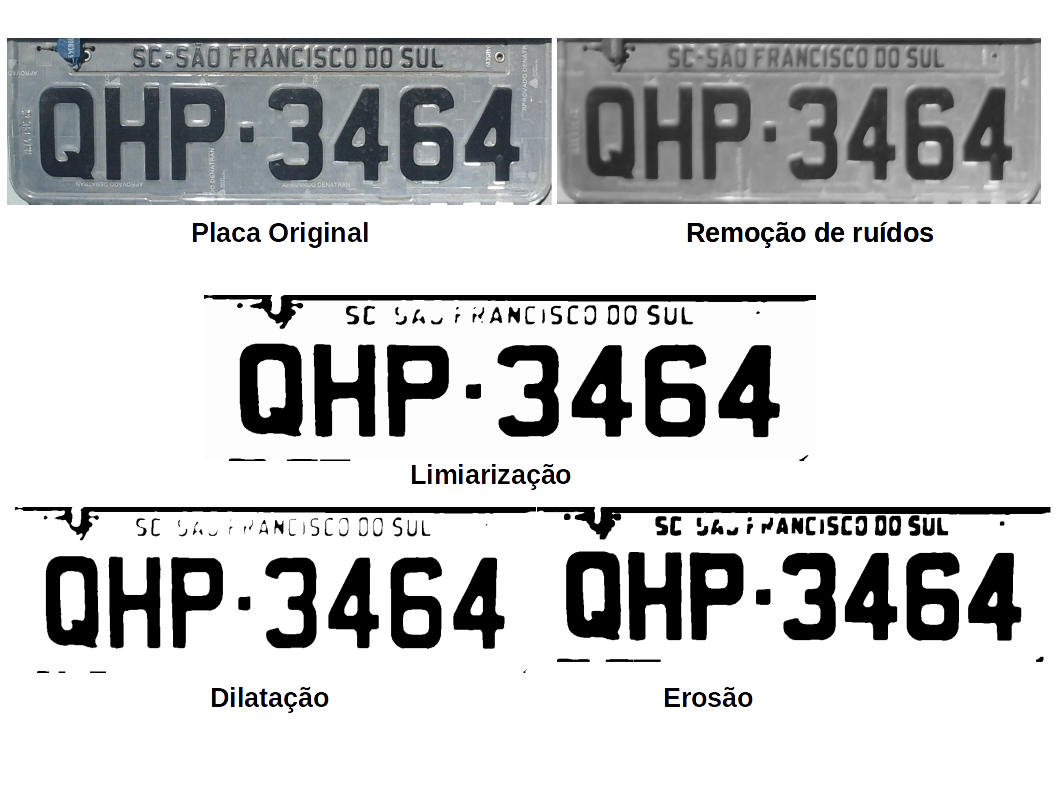
\includegraphics[width=.7\textwidth]{figuras/f1c4.png}
\end{center}
\legend{Fonte: o autor}
\end{figure}

A execução da leitura OCR através do Python é simples de fazer; basta importar a biblioteca \textit{commands} e executar o comando de leitura OCR que pode ser executado também no terminal do Linux. A biblioteca \textit{commands} permite a execução de quaisquer comandos do sistema operacional. O Código 15 é uma função de busca das saídas da leitura OCR.

\lstinputlisting[language=Python,caption={Código da Solução IV - Função de leitura OCR},label=mediapy]{codigos/implementacao3.py}

O último passo a ser dado para a implementação, é o tratamento das saídas da leitura OCR. As vezes a leitura OCR encontra pixels indesejados e os traz como resultado, o que atrapalha muito para encontrar os valores que realmente interessam. A Figura 14 representa um exemplo de um dos piores casos testados, e é de grande importancia para compreensão. É possível notar que letras que representam o nome do estado e da cidade são reconhecidos e retornados, também é perceptível que letras podem ser confundidas com números.


\begin{figure}[htbp]
\centering
\caption{Formato de respostas da leitura OCR}
\vspace{0.5cm}
\begin{tabular}{|r|c|}
\hline   
Informação da placa & SC - SÃO FRANCISCO DO SUL - MJC - 1865 & 
\hline                              
Dilatação OCRAD  &  r MJ\_C. l?Qs &
\hline
Erosão OCRAD & \_\_\_\_    \_\_\_J\_C\_ l \_\_6 5 & 
\hline
Limiarização OCRAD & MJ\_C.l?QS &
\hline
Dilatação GOCR & \_\_ \_    \_  \_ \_J\_C\_ l 8\_6 5 &
\hline
Erosão GOCR & \_\_\_\_      \_\_J\_C\_ l \_\_0 5 &
\hline
Limiarização GOCR & \_\_\_  \_\_  l \_J\_C l 8\_6 5 & 
\hline
\end{tabular}
\legend{Fonte: o autor}
\end{figure}

Na Figura 14, observa-se que na imagem que contém o filtro de dilatação, a leitura feita pelo OCRAD trouxe um pequeno ``r'' na frente do ``MJ\_C'' que são os caracteres de interesse, isso é um fator que complica muito a decisão de quais são os caracteres que realmente correspondem as letras de registro da placa, e não as de informação de estado e cidade. É possível verificar que os únicos filtros que conseguiram as letras, foram a dilatação através do OCRAD e a limiarização também pelo OCRAD, em contrapartida, os únicos filtros que conseguiram os números completos, foram os de dilatação via GOCR e limiarização também através do GOCR. Um detalhe que será explorado na conclusão, é que as letras ``MJC'' e os números ``1865'' apareceram duas vezes, e nos testes realizados, em todas as vezes que foi feita uma leitura OCR pelo menos uma vez as letras e os números apareceram em um dos filtros.

Para resolver essa situação encontrada, são necessárias duas funções, uma para encontrar as letras e outra para encontrar os números. Isso se deve a alguns erros comuns que ocorrem nas OCRs, como confundir a letra ``O'' com o número ``0''. A Figura 15 demonstra alguns dos erros mais comuns encontrados nos testes.

\begin{figure}[htbp]
\centering
\caption{Erros frequentes de leitura OCR}
\vspace{0.5cm}
\begin{tabular}{|r|c|}
\hline   
Letras & Números & 
\hline                              
O  &  0 &
\hline
l,I,i & 1 & 
\hline
B & 8 &
\hline
b, & 6 &
\hline
S,s & 5 & 
\hline
T & 7 & 
\hline
\end{tabular}
\legend{Fonte: o autor}
\end{figure}

Assumindo que esses erros apresentados são comuns, e que de maneira geral se conhece alguns erros como pontos, vírgulas, traços, interrogações e outros, a primeira ação no caso das letras é encontrar os caracteres incorretos e eliminá-los juntamente com os números, apenas deixando as letras maiúsculas. Essa limpeza resultaria nas saídas representadas na Figura 16.

\begin{figure}[htbp]
\centering
\caption{Primeira etapa de limpeza}
\vspace{0.5cm}
\begin{tabular}{|r|c|}
\hline   
Informação da placa & SC - SÃO FRANCISCO DO SUL - MJC - 1865 & 
\hline                              
Dilatação OCRAD  & MJCQ &
\hline
Erosão OCRAD & JC & 
\hline
Limiarização OCRAD & MJCQS &
\hline
Dilatação GOCR & JC &
\hline
Erosão GOCR & JC &
\hline
Limiarização GOCR & JC & 
\hline
\end{tabular}
\legend{Fonte: o autor}
\end{figure}

Nesse caso, onde houver no mínimo três caracteres, o resultado será os três primeiros, porém nem sempre os três primeiros serão as letras da placa, podendo ser uma letra da cidade ou estado como descrito anteriormente. Para os números o processo é semelhante, há uma limpeza de todas as letras e outros caracteres, deixando apenas os números e as letras que são geralmente confundidas(Figura 15) já substituídas pelo possível valor correto. No caso dos números, há uma taxa de acerto maior em relação as letras. O Código 14 demonstra um exemplo de função de limpeza para letras. Nesse código é utilizado somente a linguagem de programação, sem bibliotecas específicas para auxílio da tarefa.

\lstinputlisting[language=Python,caption={Código da Solução V - Exemplo de limpeza de letras},label=mediapy]{codigos/implementacao3-1.py}

Dessa forma, o último passo é juntar os resultados e retornar a resposta, após isso, a solução está encerrada no estágio atual. A próxima sessão tem por objetivo apresentar os resultados obtidos.

\section{Resultados}

Essa sessão apresentará os resultados parciais, considerando que a solução pode ser continuada e melhorada. 

A Tabela 1 mostra a taxa de acerto de três maneiras, sendo elas a placa completa, somente as letras e somente os números. Foram testadas trinta e cinco placas, em condições climáticas diferentes e em movimentação, fazendo uso de dispositivos móveis com no máximo oito \textit{megapixels}. A taxa de acerto pode ser considerada baixa, devido ao problema citado na sessão anterior a respeito das letras que pertencem ao estado e a cidade contidos na placa. 

Não existe um padrão de respostas, as letras podem estar em qualquer posição, misturadas entre outros conteúdos que não são de interesse. Os números também tem o mesmo problema. 

Apesar das questões citadas foram encontradas as letras e os números correspondentes a placa de maneira visual, ou seja, ao verificar as saídas OCR uma a uma, é possível identificar de que os resultados estão envolvidos nessas saídas, e isso acontece em todas as placas. 

Tendo em vista isso, uma solução seria encontrar um filtro ou efeito que de certa forma, causasse o efeito visual de embaçamento, fazendo assim com que as pequenas letras tornassem-se ilegíveis para o sistema.  

\begin{table}[htbp]
\centering
\caption{Tabela de taxa de acerto}
\vspace{0.5cm}
\begin{tabular}{|r|c|c|c|}
\hline
Descrição & Acertos & Erros & Taxa de acerto &
\hline                              
Placas completas  & 17 & 17 & 50\% &
\hline
Letras & 21 & 13 & 56.68\% &
\hline
Números & 30 & 4 & 88.23\% &
\hline

\end{tabular}
\legend{Fonte: o autor}
\end{table}

Para a questão dos números, a taxa de acerto pode ser considerada boa, obtendo quase 90\%. Aprimorar o algoritmo de decisão de números seria um passo essencial, pois alguns erros provém de letras encontradas próximas aos números, que geralmente são confundidas, como por exemplo a letra ``l'' com o número ``1''. 

Caso haja por exemplo uma saída semelhante a ``ABC l \_ ?1234'', ao limpar para encontrar apenas os números e ao substituir a letra ``l'' por ``1'', os quatro primeiros valores seriam ``1123'' e não ``1234'', e também, se esse ``l'' estivesse por entre o ``3'' e o ``4'' devido a algum pixel indejesado(que pode ser causado por ausência ou excesso de luz, ou uma série de outros fatores), o resultado seria ``1231''. Pode haver também o caso de um número não ser encontrado, obtendo apenas três números em vez de quatro.

Assim, o capítulo de desenvolvimento está finalizado, todas as conclusões e sugestões para continuação dessa solução, estarão disponíveis no próximo capítulo. O códigos que foram apresentados nesse capítulo não exatamente os que estão presentes na solução, porém como já informado no início do capítulo, nos anexos estará disponível o código completo.   
